%%%%%%%%%%%%%%%%%%%%%%%%%%%%%%%%%%%%%%%%%%%%%%%%%%%%%%%%%%%%%%%%%%%%%%%%%%%%%%%%%%%%%%%%%%%%%%%%%%%%%
%
%   Version     : 2.0
%
%   Filename    : main.tex
%
%   Description : This is the main file for the LaTeX thesis proposal document template.
%                 The template is intended for use by undergraduate students in the 
%                 BSCS major in Software Technology program.
%
%                It is assumed that you can learn how to use LaTeX on your own.
%                Please check/read the following online LaTeX book:
%
%                                 http://en.wikibooks.org/wiki/LaTeX
%     
%   Author      : Florante R. Salvador
%
%   Contributors: 1.  Karlo Campos 
%                     a. margin settings for DLSU thesis paper 
%   
%   Notes       : Please email florante.salvador@dlsu.edu.ph for comments, suggestions, ideas etc.
%
%   Reference:
%
%
%   History/Updates:
%      March 12, 2009 -- created version 1.0 for release to CSC701M (Methods of Research) students
%      May 30, 2009   -- updated Title page and Abstract for undergrad ST students
%
%      Feb 27, 2015 -- Created Version 2 (major overhaul): changed class to report, created a figures folder, 
%                               removed unnecessary packages, added new comments  based on Ethel Ong's slides
%
%%%%%%%%%%%%%%%%%%%%%%%%%%%%%%%%%%%%%%%%%%%%%%%%%%%%%%%%%%%%%%%%%%%%%%%%%%%%%%%%%%%%%%%%%%%%%%%%%%%%%%

%%%%%%%%%%%%%%%%%%%%%%%%%%%%%%%%%%%%%%%%%%%%%%%%%%%%%%%%%%%%%%%%%%%%%%%%%%%%%%%%%%%%%%%%%%%%%%%%%%%%%%%%%%%%%%%%%%%%%%%
%
%  Filename   : preamble.tex
%
%  Description: Preamble file to :
%               a. specify related packages
%               b. set margins, commands, etc.
%
%  Note       : Edit the margin settings for your own printer
%                  You may add your own commands, environments (it is assumed that you know what you're doing.)
%
%%%%%%%%%%%%%%%%%%%%%%%%%%%%%%%%%%%%%%%%%%%%%%%%%%%%%%%%%%%%%%%%%%%%%%%%%%%%%%%%%%%%%%%%%%%%%%%%%%%%%%%%%%%%%%%%%%%%%%%

%\documentclass[12pt,titlepage,onepage, letterpaper]{article}

\documentclass[12pt,titlepage,onepage, letterpaper]{report}


%
%-- specify related packages
%

%
% \usepackage[utf8x]{inputenc}
%

\usepackage{apacite}           %-- APA style citation 
                               %-- refer to http://www.ctan.org/tex-archive/biblio/bibtex/contrib/apacite/

%
%  \usepackage{ucs}
%


\usepackage{amsmath}           %-- American Math Society packages
\usepackage{amsfonts}
\usepackage{amssymb}
\usepackage{pdflscape}

\usepackage{graphicx}          %-- graphicx package needed for including figures in JPG or PNG format
 
%
%\usepackage{graphics}          %-- graphics related package (this was commented out) use when image is in EPS format
%

\usepackage{verbatim}          %-- this package allows you to have multiple lines of comments by
                               %-- example:
                               %   \begin{comment}
                               %        ...your text here...
                               %   \end{comment}  

\usepackage{color}             %-- allows use of color with text
                               %-- example:  \textcolor{red}{This is the colored text in red.}

\usepackage{url}  %-- allows use of URLs example: \url{https:\ccs1.dlsu.edu.ph}


%
%-- set margins,  you may need to edit this for your own printer
%
\topmargin 0.0in
\oddsidemargin 0.0in
\evensidemargin 0.0in

\voffset 0.0in
\hoffset 0.5625in

\textwidth 5.75in
\textheight 8.5in


\parskip 1em
\parindent 0.25in

\bibliographystyle{apacite}            %-- use APA citation scheme

\hyphenation{ana-lysis know-ledge}     %-- LaTeX may not hyphenate correctly some words you use in your document
                                       %-- use \hyphenation to instruct LaTeX how to do it correctly, example above

\newcommand{\degree}{^{\circ}}         %-- use \newcommand to create your own "commands"
                                       %-- \newcommand works like the #define you learned in your COMPRO1 class

\newcommand{\etal}{et al.}


%\newcommand{\sinag}{\emph{Sinag}}
%\newcommand{\sinagtwo}{\emph{Sinag2}}

\newcommand{\figref}[1]{Figure \ref{#1}}
\newcommand{\appref}[1]{Appendix \ref{#1}}

%-- \newcommand{\Section}[1]{\section{#1}\setcounter{figure}{0}\setcounter{table}{0}}

%\newcommand{\shade}{\multicolumn{1}{|>{\columncolor[gray]{0.25}}c|}{}}
%\newcommand{\tableheader}[1]{\rowcolor{black}\color{white}{#1}}
%\newcommand{\cell}[2]{\multicolumn{1}{#1}{#2}}
%\newcommand{\definition}[2]{\textbf{\textit{#1}} --- #2}
%\newcommand{\itembit}[1]{\item \textbf{\textit{#1}}}
%\newcommand{\sgdef}[2]{\parbox[t][][t]{1.75in}{\textbf{#1}} \> \parbox[t][][t]{4.0in}{#2}\\\\}

%\newenvironment{sinagglossary}{\begin{flushleft}
%\begin{tabbing}
%\hspace{1.75in}\=\\}{\end{tabbing}\end{flushleft}}

\newcommand{\thestitle}[1]{{\Large \textsc{#1}}}


%---
%  \renewcommand{\thefigure}{\thesection.\arabic{figure}}
%  \renewcommand{\thetable}{\thesection.\arabic{table}}
%  \renewcommand{\contentsname}{Table of Contents}


                %-- includes LaTeX source file for the preamble 
                                  %-- include packages, sets the margin sequence, and many more... 
                                  %-- your job: check if the settings are suitable for your own printer

\graphicspath{{figures/}}  %-- figures is the name of the folder containing images JPG or PN

\begin{document}

%%%%%%%%%%%%%%%%%%%%%%%%%%%%%%%%%%%%%%%%%%%%%%%%%%%%%%%%%%%%%%%%%%%%%%%%%%%%%%%%%%%%%%%%%%%%%%%%%%%%%%
%
%   Filename    : title_page.tex 
%
%   Description : This file will contain your Title Page.
%                 
%%%%%%%%%%%%%%%%%%%%%%%%%%%%%%%%%%%%%%%%%%%%%%%%%%%%%%%%%%%%%%%%%%%%%%%%%%%%%%%%%%%%%%%%%%%%%%%%%%%%%%

\begin{titlepage}
\centering


%-- **EDIT** the following line to indicate your thesis title
\thestitle{Visual Feedback for Speech Training Aiding the Hearing-impaired in Learning Diphthongs with Consonants}

\vspace{1.75cm}
A Thesis Proposal\\
Presented to\\
the Faculty of the College of Computer Studies\\
De La Salle University Manila

\vspace{1.75cm}
In Partial Fulfillment\\
of the Requirements for the Degree of\\

Bachelor of Science in Computer Science

\vspace{1.75cm}
by\\
%-- **EDIT** the following line to indicate your name 
\vspace{1cm}

CABERIO, Aldrin  \\
CRUZ, Lelis  \\
FLORES, Joshua  \\
LIM, David  \\

\vspace{1.75cm}
%-- **EDIT** the following line to indicate your adviser's name 
Solomon SEE \\
Adviser

\vspace{1.75cm}
\today
\end{titlepage}
              %-- includes LaTeX source file for the Title Page 
                                  %-- your job: **EDIT THIS FILE ** to indicate your own title, name, and thesis adviser's name
%%%%%%%%%%%%%%%%%%%%%%%%%%%%%%%%%%%%%%%%%%%%%%%%%%%%%%%%%%%%%%%%%%%%%%%%%%%%%%%%%%%%%%%%%%%%%%%%%%%%%%
%
%   Filename    : abstract.tex 
%
%   Description : This file will contain your abstract.
%                 
%%%%%%%%%%%%%%%%%%%%%%%%%%%%%%%%%%%%%%%%%%%%%%%%%%%%%%%%%%%%%%%%%%%%%%%%%%%%%%%%%%%%%%%%%%%%%%%%%%%%%%

\begin{abstract}
From 150 to 200 words of short, direct and complete sentences, the abstract should be informative enough to serve as a substitute for reading the thesis itself.  It states the 
rationale and the objectives of the research.  In STTHES3, i.e., final thesis stage, the 
abstract should also contain a description of your research results/findings/contribution(s).

%
%  Do not put citations or quotes in the abract.
%

  
Keywords can be found at \url{http://www.acm.org/about/class/1998/}.  Click the link to 
``single HTML document'' or ``browsable HTML document...''.

\begin{flushleft}
\begin{tabular}{lp{4.25in}}
\hspace{-0.5em}\textbf{Keywords:}\hspace{0.25em} & Keyword 1, keyword 2, keyword 3, keyword 4, etc.\\
\end{tabular}
\end{flushleft}
\end{abstract}


\pagenumbering{roman}             %-- this will number pages as i, ii, iii, etc...
\setcounter{page}{2}

\newpage

\pagenumbering{arabic}            %-- this will number pages as 1, 2, 3, etc...
\setcounter{page}{1}              

\chapter{Research Description}
\label{sec:researchdesc}

This chapter discusses the overview of the current state of technology, research objectives, scope and limitations of the research, and significance of the research.

\section{Overview of the Current State of Technology}
\label{sec:overview}

Hearing impairment is the inability to hear, and it may affect one's development when learning how to speak \cite{lasak:2014:HL}. Some people are born with hearing impairment, and some obtain it due to age, illness, trauma, and other factors. An extremely deaf child may find it immensely difficult to learn speech and language without auditory feedback \cite{bernstein:1988:STA}.

\begin{comment}
Throughout the years, man has tried to find ways to help the hearing-handicapped learn how to speak properly \cite{oyer:1976:CHH}. Oyer \citeyear{oyer:1976:CHH} states that there was a time when hearing-handicapped were considered unfit to hold citizenship. James Pickett, a professor of speech communication research says "I believe that large improvements in the lives of deaf persons depends on making large improvements in their speech communication" \cite{connor:1971:SDC}. Pickett also states that in the late 19th century, research began for helping the Deaf communicate \cite{connor:1971:SDC}.

One problem of a hearing-impaired student is the lack of access to speech training aids outside of therapy \cite{bernstein:1988:STA}. Extensive practice is required for the student to progress \cite{bernstein:1988:STA}.
\end{comment}

Early speech training software were implemented using a lip reading technique, wherein the systems take the user's lip movement as input \cite{heracleous:2010:CSA}. However, many phonemes share similar facial and lip shape (visemes) with other phonemes as well; resulting to phonemes not being discernable through visual data alone \cite{heracleous:2010:CSA}.

Bernstein et al. \citeyear{bernstein:1988:STA} mentions that visual information is commonly practiced to aid in speech perception. Several visual displays were designed to grasp the attention of children wherein they play games to learn. One of such games is a 'ball game' wherein the ball changes in size depending on the loudness of the sound the child makes. The ball also can be controlled going to the hoop using the child's voice pitch \cite{bernstein:1988:STA}. Another game is a vertical spectrum, which is visually displayed as a changing 2-dimensional shape wherein frequency was displayed on the y-axis, and amplitude---the degree of change---on the x-axis \cite{bernstein:1988:STA}.

Currently, one way for a hearing-impaired person to learn how to speak is by planting an electronic device called a cochlear implant. It is designed to function as a cochlea, a part of the ear which receives sounds in the form of vibrations and these vibrations are sensed by hair cells. Deaf people are unable to hear because their hair cells cannot detect the vibrations as received by the cochlea due to damaged hairs cells, or they have less hair cells. Cochlear implants stimulate the cochlear nerves without going the hair cells anymore. A person with a cochlear implant may still undergo training and therapy in order to adjust to their hearing \cite{blume:2009:AE}. Once a person hears properly, it can lead to speech training and therapy in order for one to respond accordingly to different sounds.
					
Computer-based speech therapy systems that have been implemented are mostly product-oriented, providing an analysis of the input of the user and the final result. The method, however, does not provide the information of how the sound should be articulated. The shortcoming of these systems are brought upon by giving visual representations in real time i.e. game-like visualizations and speech pictures \cite{oster:2006:cbs}.
									
Moreover, in training hearing-impaired children, the most preferred feedback is through visual modality. This allows the children see the motor gestures that were non-visible, assisting them in developing their speech gestures. The problem that this method posed was that it was seldom evaluated in a pedagogical programme. Often, the visual aids presented was difficult to understand, unnatural, delayed, unattractive, and had no motivational impact on the children \cite{oster:2006:cbs}.
				
\section{Research Objectives}
\label{sec:researchobjectives}

\subsection{General Objective}
\label{sec:generalobjective}

To implement a speech training software that provides visual feedback to assist people with hearing impairment in order to learn how to speak vowel sounds.

\subsection{Specific Objectives}
\label{sec:specificobjectives}

\begin{enumerate}
\item To study how previous and current speech training programs work
\item To find Deaf schools who may assist the proponents with the research
\item To identify and compare different methods of visual feedback in speech training systems
\item To select the optimal visual feedback method based on usability and effectiveness
\item To review Natalie Agustin's \citeyear{agustin:2014:SOM} master's thesis, a mapping program which will be integrated into the speech training software
\item To determine the different methods in motivating the hearing-impaired in using the speech training software
\item To evaluate the accuracy of the speech training software's visual feedback based on the user's voice input
\end{enumerate}

\section{Scope and Limitations of the Research}
\label{sec:scopelimitations}

For the implementation of the speech training software, the master's thesis of Natalie Agustin \citeyear{agustin:2014:SOM} will be used. Agustin's program is a mapping software which receives voice input from the user and identifies the vowel sound made by the user and displays the user’s articulation---the movement of the lips, tongue, jaw, and other speech organs. Agustin's thesis will be used for the system to know which vowel the user had spoken.
The speech training software will be written in Java, a cross-platform programming language, making the system usable by different operating systems.
The speech training software will run on a desktop platform, as desktop computers are accessible and widely-used.

\section{Significance of the Research}
\label{sec:significance}

The thesis will assist the Deaf in learning the pronunciations of vowel sounds correctly. Deaf communities may make use of the software, guided by a professional speech trainer, in his or her development with regard to speech training.
The thesis may serve as a basis for future implementations of Deaf speech training software which may cater not only vowels, but also consonants.
%%%%%%%%%%%%%%%%%%%%%%%%%%%%%%%%%%%%%%%%%%%%%%%%%%%%%%%%%%%%%%%%%%%%%%%%%%%%%%%%%%%%%%%%%%%%%%%%%%%%%%
%
%   Filename    : chapter_2.tex 
%
%   Description : This file will contain your Review of Related Literature.
%                 
%%%%%%%%%%%%%%%%%%%%%%%%%%%%%%%%%%%%%%%%%%%%%%%%%%%%%%%%%%%%%%%%%%%%%%%%%%%%%%%%%%%%%%%%%%%%%%%%%%%%%%

\chapter{Review of Related Literature}
\label{sec:relatedlit}

This chapter discusses studies for an effective speech training system and different software that have been distributed and used by the hearing-impaired in order to learn how to speak.

\section{Review of Related Paper}

\subsection{Speech Training Systems}

Speech is not innate for children who are deaf or with a profound hearing loss at birth. The effect of such disability obstructs a child from imitating other people’s sounds and comparing the sound he/she may be able to produce with theirs. However, the development which can’t be learned through spontaneous speech could be acquired through vision, tactile sensation, and residual hearing. Although, this learning method solely relies on the visual representation of phonemes and through tongue control movements in sustaining the speech movements. Computer-based speech therapy aided programs makes use of visual feedbacks to allow individuals with profound hearing impairments to evaluate themselves with their produced input compared with an acceptable input. By garnering the attention of the children through drawings and illustrations to demonstrate loudness, pitch contour, spectral distribution, etc., they are able to validate their produced sound \cite{oster:2006:cbs}.

Speech Training Systems were developed in order to represent feedback to people with profound hearing impairment in a visually appealing manner \cite{oster:2006:cbs}. Other implementations of software address this solution by introducing gamifying elements to allow the software to be used by the direct users or under the assistance of teachers. Methods such as spectrographs, dating since 1947, have also been used to teach speech to children \cite{javkin:1993:msa}. On the other hand, tactile aid focuses on somatosensation; by using vibrators at various parts of the body to indicate numerous elements of speech such as voicing or nasalization \cite{wankhede:2014:dvs}.

Strategies are often required in implementing such systems, especially to deaf children, who necessitates more efficient methods of instructions compared to hearing children. Speech training is efficient if it would be able to allow children to imitate invisible speech articulations, which could not be perceived properly by visual aids \cite{oster:1996:cac}. Oster \citeyear{oster:1996:cac} suggests that for a speech training system to considered efficient and to able to amplify the any possibility for a child to learn, a number of requirements must be achieved:

\begin{itemize}
\item “Clear instructions and pedagogical manuals must be created and made available for use with different groups of children.
\item The visual feedback of the child’s voice and articulation should be shown immediately and without delay.
\item The aid must be acceptable to the therapist as well as to the child, which means that the aid must be attractive, interesting, easily comprehensible, easy to handle, and motivating.
\item The visual pattern must be natural, logical and easily understandable. This means that training parameters as, e.g., pitch could be shown vertically as pitch variations occur; intensity through the size of an object that becomes larger as a sound becomes louder and smaller as a sound becomes softer; intonation and stress through a continuous red curve; duration could be shown horizontally and voicing through a relationship between voicing and the change of a colour.
\item The aid should provide a contrastive training, that is, the correct model of the therapist and the deviant production of the child are shown simultaneously and compared with each other.
\item The aid should provide a flexible, individual, and structural speech and voice training and give an objective evaluation of the child’s training results.” \cite{oster:1996:cac}
\end{itemize}

A speech training system that provides visual aid will help a hearing-impaired person evaluate and correct his utterance or pronunciation \cite{wankhede:2014:dvs}. Wankhede mentions that how the feedback is presented also affects how hearing-impaired children may improve their pronunciations. The visual feedback must also be shown immediately on the computer screen without delay to prevent confusion to the child. Some children may find some speech training aids as difficult to understand, unnatural, delayed, unattractive, and unmotivating to the children. For evaluation of the speech training aid, it should have the acceptance of a speech therapist and as well as of a child, meaning that the system should be appealing, presentable, easy to use, and motivating \cite{wankhede:2014:dvs}.

Aside from visual feedback that are used as aid in speech training system, there is also another type of feedback being used as aid for the hearing-impaired people in speech training - vibrotactile feedback. The Haptic Chair is a project developed by Suranga Nanayakkara, Lonce Wyse, and Elizabeth A. Taylor, to help deaf people in speech training by the use of sending vibrotactile feedback to several parts of the body such as palm and fingers \cite{nanaya:2012:hap}.

\subsection{Self-Organizing Maps (SOMs)}

Self-organizing map (SOM) is an artificial neural network that discovers patterns in the input data and can learn even without supervision \cite{agustin:2014:SOM}. The input is then transformed into a one or two dimensional map and a weight is given to it and perform this transformation adaptively in a topologically ordered fashion \cite{chandar:2013:srs}.

SOMs have neurons or nodes in which each node/neuron has a weight that is similar in dimension as the input and these nodes are then arranged in the map to from a hexagonal or rectangular grid, connecting them to each input node \cite{agustin:2014:SOM}.

At the start, the neurons are given random weight values. This is called the initialization phase. The next step of the process is determining which neuron is closest to the input via its given weight value. “The weights of the winning neuron and neurons close to it in the SOM lattice are adjusted towards the input vector” \cite{chandar:2013:srs}. This is called the competition phase \cite{agustin:2014:SOM}. Lastly, the weight of the winning neurons and its neighbors are adjusted in relation to the input pattern in this third phase called adaptation phase, hence, the SOM is created.               %-- includes LaTeX source file for Chapter 1: Research Description
                                  %-- your job: **EDIT THIS FILE** to indicate your own research description
%%%%%%%%%%%%%%%%%%%%%%%%%%%%%%%%%%%%%%%%%%%%%%%%%%%%%%%%%%%%%%%%%%%%%%%%%%%%%%%%%%%%%%%%%%%%%%%%%%%%%%
%
%   Filename    : chapter_3.tex 
%
%   Description : This file will contain your Theoretical Framework.
%                 
%
%%%%%%%%%%%%%%%%%%%%%%%%%%%%%%%%%%%%%%%%%%%%%%%%%%%%%%%%%%%%%%%%%%%%%%%%%%%%%%%%%%%%%%%%%%%%%%%%%%%%%%

\chapter{Theoretical Framework}
This section discusses relevant theories and concepts to be used in the course of designing or developing the thesis.

\section{Speech Theory}

\subsection{Phonetics}
Phonetics focuses on the study of speech sounds, physiological production and their acoustic qualities. It is comprised of three branches. Articulatory Phonetics deals with the movement of the vocal organs that produces speech sounds. Acoustic Phonetics pertains to the acoustic properties of speech sounds; how the sound is being transmitted from the speaker to the listener. Lastly, Auditory Phonetics refers to the reception and perception of the listener \cite{britannica:2014:phoetics}.

\subsubsection{Articulatory Phonetics}
The traditional method of describing the physiological production of sound is through the vocal organs that produces them. The production of sound requires the use of the lungs, respiratory system, altogether with the vocal cords.

Speech sounds are separated into two major divisions, vowels and consonants. Vowels includes sounds that are produced without any major constrictions in the vocal tract. In the formation of consonants however, the airstream though the vocal tract is obsturated in a certain way \cite{britannica:2014:phoetics}.

\subsubsection{Acoustic Phonetics}
% Source: http://www.britannica.com/science/phonetics/Acoustic-phonetics

\begin{figure}[ht]
    \centering
    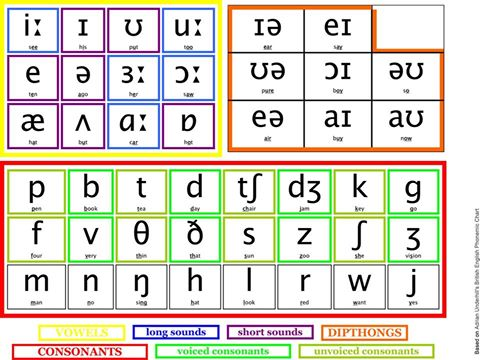
\includegraphics[totalheight=0.2\textheight]{diphthong-chart.jpg}
    \caption{Blue, J. (2013). }
    \cite{usingphonemes:img}
    \label{fig:diphthong-chart}
\end{figure}

Sounds that are produced by individuals differ from one another; varying in pitch, loudness, and quality. There are certain types of sounds that consists of periodic waves, one of which is the voiced sound. A voiced sound's pitch is determined in its fundamental frequency, or rate of repetition of the cycles of air pressure. The loudness of the voiced sound is dependent on the amplitude of the pulses of air pressure produced by the vibrating vocal cords. Pulses of air with a larger amplitude have a larger increase in air pressure. The smaller vibrations help determine the quality of a sound. Moreover, these smaller variations in air pressure correspond to the overtones that occur above the fundamental frequency \cite{britannica:2014:acoustic-phoetics}. 

\subsection{Phonemes}
Phonemes are singular units of sound. These set of units are comprised of all the vowels and consonants in the English alphabet, arranged and grouped according to their characteristics \cite{wikipedia:2014:phoneme}. Phonemes are categorized into two classes: Vowels, Consonants. Vowels are further divided into two classes, monothongs, which is subdivided into long ang short vowel sounds, and diphthongs. Consonants are also split into two categories, the unvoiced consonants and the voiced consonants \cite{jadeblue:2013:phonemic-chart}. 

\subsubsection{Diphthongs}
In linguistics, diphthongs, also known as gliding vowels, are a combination of two different vowel sounds. Compared to vowel sounds, diphthongs occur when a vowel sound is produced and the tongue moves during the pronunciation of the aforementioned vowel \cite{britannica:2015:diphthongs}.

\section{Feedback Mechanisms}

Feedback is considered either a positive or a negative one. A positive feedback is called "positive reinforcement" while a negative feedback is called "punishment" \cite{brookhart:2008:gef}. These feedback theoretically affect learning; however, not all feedback are effective \cite{brookhart:2008:gef}.


\begin{comment}
\begin{table}[!htbp]   %t means place on top, replace with b if you want to place at the bottom
\centering
\caption{Table of Feedback Strategies} \vspace{0em}
\begin{tabular}{|p{1in}|p{1.5in}|p{2in}|}
 \hline
\centering
Feedback Strategies May Vary In... & In These Ways... & Recommendations for Good Feedback \\ \hline
    Timing
    & \begin{itemize}
        \item When given
        \item How often
      \end{itemize}
    & \begin{itemize}
        \item Provide immediate feedback for knowledge of facts (right/wrong).
        \item Delay feedback for more comprehensive reviews of student thinking and processing.
        \item Never delay feedback when it would make a difference to students.
        \item Provide feedback as often as is practical, for all major assignments.
        \end{itemize}
        \\ \hline
    Amount
    & \begin{itemize}
        \item How many points made
        \item How much about each point
        \end{itemize}
    & \begin{itemize}
        \item Prioritize - pick the most important points.
        \item Choose points that relate to major learning goals.
        \item Consider the student's developmental level.
        \end{itemize}
        \\ \hline
    Mode
    & \begin{itemize}
        \item Oral
        \item Written
        \item Visual Demonstration
        \end{itemize}
    & \begin{itemize}
        \item Select the best mode for the message Would a comment in passing the student's desk suffice? Is a conference needed?
        \item Interactive feedback (talking with the student) is best when possible.
        \item Give written feedback on written work or on assignment cover sheets.
        \item Use demonstration if "how to do something" is an issue or if the student needs example.
        \end{itemize}
        \\ \hline
    Audience
    & \begin{itemize}
        \item Individual
        \item Group/class
        \end{itemize}
    & \begin{itemize}
        \item Individual feedback says, "The teacher values my learning."
        \item Group/class feedback works if most of the class missed the same concept on an assignment, which presents an opportunity for reteaching.
        \end{itemize}
        \\ \hline
\end{tabular}
\label{tab:feedback-strategy-table}
\end{table}
\end{comment}

\begin{figure}[ht]
    \centering
    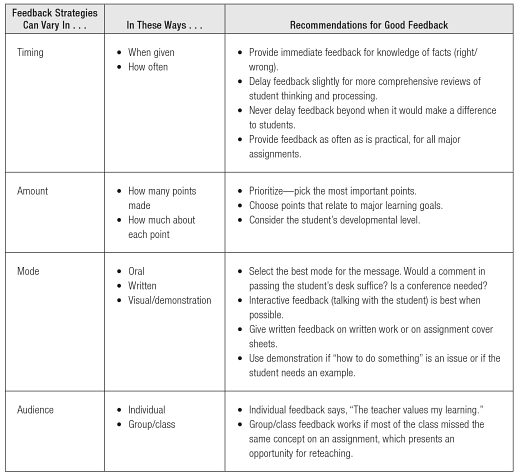
\includegraphics{feedback-strategy-table.PNG}
    \caption{Feedback Strategies Table (Brookhart, 2008)}
    \label{fig:feedback-strategy-table}
\end{figure}

Certain strategies are used to give feedback in different ways. These strategies may vary in Timing, Amount, Mode, and Audience while the feedback content may vary in focus, comparison, valence and other variations \cite{brookhart:2008:gef}. Timing strategy refers to when a feedback should be given and how often it should be given. A feedback may be given immediately if the output needed is factual or may be delayed if it requires more analysis. Generally, the feedback should be given as often as needed. Amount of feedback to be given to the students depending on how many important points are needed, for example, if a student is learning speech, certain points to consider are the accent and the grammar of the student. The mode of showing the feedback varies in oral, written or visual demonstration. Interactive feedback are considered best, which means it relates the performance of the student to actual task. Audience refers to how many students are receiving feedback. It may be individual or in a group or class. Individual feedback makes the student realize that the teacher is focused on their learning while group or class feedback is best used when most of the class have the same misunderstanding which may lead to reteaching.

The use of different feedback strategies depend on which part a student should improve on or when it should be given as shown in \figref{fig:feedback-strategy-table}. 

\subsection{Mode Strategy}
Feedback in a form of mode may be shown in oral, written or other visual demonstration. One visual demonstration may be used is showing it in a "how it should be done" form. It may be demonstrated by a person or by a video playback.

% FEEDBACK, MORE THAN JUST YES AND NO
% How are people visualising it?
\subsection{Traditional Methods}
% What are traditional ways & methods?

\begin{comment}
Various ways to teach speech to the deaf were invented and developed since it was pioneered in the 16th century \cite{markides:1983:sohic}. It started with Pedro Ponce de Leon, a Benedictan monk in Spain, who first started teaching speech to the Deaf when he met two deaf boys and was put under the care of the monastery \cite{markides:1983:sohic}.
\end{comment}

Currently, traditional ways of teaching speech requires the aid of a speech therapist and not only teach children with hearing-impairment how to speak but also children with Down syndrome, motor speech disorders, developmental delays and other speech disorders. Various speech therapies may be used depending on the disorder the child has. A speech therapy's purpose is to systematize the mechanics of speech with the use of language and it is often included in autism behavioral intensive programs \cite{autispks:2015:slmi}. Developmental verbal dyspraxia, a disorder that makes a child unable to speak sounds and words well, may also be managed by a different type of speech-language therapy. Aphasia is another condition wherein a person is having difficulties in speaking due to brain damage \cite{damasio:1992:aphasia} which happens after a person had experienced stroke. Speech therapy helps them by giving drills to improve specific language skills, group therapy to improve conversational skills, and augmenting their communication skills through gestures and writing \cite{hayes:2013:tost}.

Other conditions and disorders that may be treated by speech therapy, as listed by Hayes \citeyear{hayes:2013:tost}, are stuttering, swallowing difficulties, and children who are late talkers.

\subsection{Speech Training for the Hearing-Impaired}
Speech Training systems that were previously implemented focused on the visual stimuli of the Deaf students in order to learn speech. However, the method of providing feedback differed from one software to another, only dealing with a certain topic for the student to learn.

The software SpeechViewer III, developed by IBM, was created to develop the vocal skills of the hearing-impaired \cite{speechville:2014:slp}. By transforming a user's speech to a graphically represented model, the students are motivated to continue developing their voicing, pitch, loudness, phoneme accuracy and speech timing \cite{kennedy:1998:spv}.

Similarly, Speech Therapy 5, offers the same capabilities of SpeechViewer 3. However, it has expanded to over 70 types of games, allowing the student to futher practice speech. Speech Therapy 5 has also allowed the student's supervisors to provide additional feedback as the program provides graphical display and statistical data of the students's performance \cite{drspeech:1998:st5}.

Video Voice, another speech training system that has been providing assitance to hearing-impaired indivuals for more than 35 years, has expanded its faculties by accomodating almost any type of speech work \cite{videovoice:2015:description}. Video Voice also displays its feedback by means of a gamified graphical representation of an individual's speech \cite{videovoice:2015:speechtherapyapplications}. In addition, Video Voice renders formants for every individual, displaying their performances on various models in order for their therapists to select the appropriate therapy targets \cite{videovoice:2015:formantdisplays}.

\subsection{Speech Training for Children}

Numerous Speech Training systems and methods, in both computerized and traditional, have been constructed to benefit other individuals with different disablities or impairments. 

A system has been developed in order to cater the needs of language-learning impaired children, who are having difficulty in learning their native language. Through the use of an algorithm that renders the volume of rapidly change elements in speech, to make them salient, they futher improved on their performance \cite{jstor:1996:lli}. Schizophrenic Children on the other hand were taught through series of verbal discrimination, being rewarded as they are able to replicate the adult's speech \cite{science:1966:schizo}.

Through the use of the picture exchange communication system (PECS), an augmented and alternative communication, allows children with autism to learn communication by means of exchanging pictures for items or activites they are interested in \cite{wiley:2002:pictureexchange}. 

Children with spoken language impairment (SLI) often shows signs of early reading delay. Such impairment demonstrated expressive phonological difficulties, more so, had retarded development of their semantic and syntactic skills \cite{lshss:2000:sli}. Through the introduction of the integrated phonological awareness intervention to these preschool children, it has assisted them in developing their speech. with spoken language impairment, students undergo series of speech production, phonological awareness and letter-sound knowledge \cite{gillonmcneill:2007:sli}.

Bungalow Software, is a speech and language recovery system for patients recuperating from after stroke traumatisation, aphasia, or brain injury. This software was designed to work a way such that a speech pathologist is providing series of drill therapies to the patient. Series of questions is asked to the patient, where they will have to try answering each question until they provide the correct answer. By instant grading and giving hints to the patients, they are motivated and are able to learn faster \cite{bungalow:2012:speechtherapy}.

\subsection{Accent Traning}
% Call Center Agent Accent Training
Accent is simply defined as a distinctive way of speaking speech sounds and it is associated within a certain group or nation \cite{adams:2009:sgsa}. Some people attempt to change their accents to improve within the field of their work \cite{ravin:2004:lyad}. Currently, one may get accent trainings through online courses or with the aid of self-help books such as Jennifer Adams and Johanna Chapman's \citeyear{adams:2009:sgsa} and Judy Ravin's \citeyear{ravin:2004:lyad} books.

Generally, a person may change or imrpove their accent by surrounding themselves with people having the accents they want to acquire and listen to them closely \cite{omniglot:2015:ttiya}. Another is by attempting to speak in that target accent which may be practiced by reading sentences aloud or listening to a practice module consistently \cite{omniglot:2015:ttiya}. Courses and books train students to a more focused scope in the accent. It usually starts with speaking certain vowels and consonants using the target accents and linking the vowels and consonants together and, finally, applying it to conversations and informal speech \cite{ravin:2004:lyad}.

% --------- CS FRAMEWORK ---------

\section{Self-Organizing Maps (SOMs)}
Self-organizing map (SOM) is an artificial neural network that discovers patterns in the input data and can learn even without supervision \cite{kohonen:1988:pho}. It transforms multi-dimensional inputs into a two-dimensional mapping and each output in the map is given a weight \cite{chandar:2013:srs}. SOMs may be used to detect or map a vowel sound based on a user's voice input. 

The map consists of grid of squares called "nodes". Each node is equivalent to a category (or a combination of the different dimensions of data depending on the intensity of each dimension). It is also ensured that topology is reserved which means that a node has a great relation between other neighboring nodes \cite{li:2008:som}.

At the start, the neurons are given random weight values. This is called the initialization phase. The next step of the process is determining which neuron is closest to the input via its given weight value. "The weights of the winning neuron and neurons close to it in the SOM lattice are adjusted towards the input vector" \cite{chandar:2013:srs}. This is called the competition phase \cite{agustin:2014:SOM}. Lastly, the weight of the winning neurons and its neighbors are adjusted in relation to the input pattern in this third phase called adaptation phase, hence, the SOM is created.

% The input of the her thesis is not sound, but processed sound or audio which is converted to CSV.
\begin{comment}
For example, considering Natalie Agustin's \citeyear{agustin:2014:SOM} thesis, the input of the system would be sound or audio, specifically vowel sounds from the user's voice. The 5 basic vowel sounds ('a', 'e', 'i', 'o', 'u') are considered to their own nodes (category) and everything else in between (i.e. combination of 'a' and 'e' sound or longer 'oo' sound) will have their own nodes as well. The basic vowels are identified as the different dimensions, meaning we have 5-dimensional data. Once the system read an input, it will weigh in each dimension to the input and will be mapped accordingly to a node.
\end{comment}

\section{Mel-Frequency Cepstral Coefficients (MFCC)}
% Still incomplete. Add info about the other steps but not too detailed.
The Mel-Frequency Cepstral Coefficients (MFCC) is common for translating speech sound into coefficients and has succeeded because of representing the speech amplitude spectrum in a compact form \cite{logan:2000:mel}. Out of all existing feature extraction models, MFCC is the most popular and has become the standard in speech recognition systems \cite{Sahidullah2012543}. MFCC is a good feature extraction model as it discards unneeded data (background noise, emotion, etc).

This feature extraction model generally consists of five steps: Windowing, Taking the Discrete Fourier Transform (DFT), Applying the Mel Filterbank, Taking the Log of All Filterbank Energies and Taking the Discrete Cosine Transform.

The windowing step divides the audio into several windows and is described more in detail in the following subsection. The DFT extracts which frequencies are present from each frame. However, the output of the DFT still contains unneeded information for speech recognition which is why each frame goes through a filterbank which outputs how much energy exists in each frequency band. Taking the log from each filter from the previous step allows usage of ceptral mean subtraction, a channel normalisation technique. The final step computes the DCT of the log filterbank energies which outputs the Mel-Frequency Cepstral Coefficients.

\subsection{Windowing}
In this step, the audio is divided into several windows, each having an interval of usually 20 milliseconds (also called the frame size). Each window is statistically stationary, making feature extraction less complex as the sounds of each window are static.

The problem with speech is that it is not stationary, sound and pitch change throughout the speech, thus may face issues when performing the latter parts of the MFCC model. The windowing step is designed to make the speech (or parts of the speech) stationary by dividing it into windows. There are configurations before performing windowing. First, the frame size is to be determined. The frame size defines how long (in milliseconds) a frame is. Usually, 20 milliseconds is set as the frame size \cite{han:mfcc-extraction:2006}. Second, the frame shift is also to be determined. The frame shift is the offset between windows \cite{agustin:2014:SOM} and is usually set to 10 milliseconds \cite{han:mfcc-extraction:2006}.

\begin{figure}[h]
    \centering
    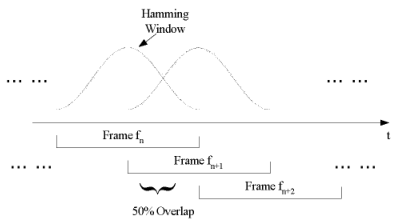
\includegraphics{hamming-window.PNG}
    \caption{Frame blocking in the MFCC extraction algorithm (Han et al., 2006)}
    \label{fig:hamming-window}
\end{figure}

One issue present when cutting audio into several windows is that these windows are snipped instantly, causing high frequency noises at each frame's start point and end point due to sudden change \cite{han:mfcc-extraction:2006}. The Hamming window is used to reduce or stabilize a frame's frequency noise. As shown in \figref{fig:hamming-window}, the maximum height of a frame is similar to the other frames.

\section{Agustin's Research}
Natalie Agustin's research uses Self-Organizing Maps and regression models in order to display Visual Articulatory Feedback (VAF). Agustin's VAF displays how articulations---speech organs which produce sound---are formed when pronouncing a vowel. Agustin's software prototype takes audio (vowel pronunciation) as input and outputs the VAF. Models created in her research are from the MOCHA-TIMIT dataset, which were created by The University of Edinburgh's Centre for Speech Technology Research. The MOCHA-TIMIT dataset provides a phonetically balanced dataset for training an automatic speech recognition system. The VAF is shown in side view, displaying vocal tracts on a shape of a face drawn on a plotted Cartesian map.

Agustin's purpose for the research was to create a VAF system for speech learning of people with hearing impairment. Agustin developed a prototype which visually displays the articulations that need to be formed in order to speak the targeted sound.

Agustin has provided the researchers of this paper with her method of training data with the use of EMA files from the MOCHA-TIMIT dataset. This will allow the researchers to change the dataset, that instead of vowels, consonant-diphthongs will be used. Also, the SOM algorithm by Agustin will be used by the researchers as well which will be needed in the feedback system in determining how far or how near the trainee is from the targeted pronunciation.
%%%%%%%%%%%%%%%%%%%%%%%%%%%%%%%%%%%%%%%%%%%%%%%%%%%%%%%%%%%%%%%%%%%%%%%%%%%%%%%%%%%%%%%%%%%%%%%%%%%%%%
%
%   Filename    : chapter_4.tex 
%
%   Description : This file will contain your The Speech Feedback System.
%                 
%%%%%%%%%%%%%%%%%%%%%%%%%%%%%%%%%%%%%%%%%%%%%%%%%%%%%%%%%%%%%%%%%%%%%%%%%%%%%%%%%%%%%%%%%%%%%%%%%%%%%%

\chapter{SpeechViz}
This section gives the overall specifications and functional requirements of the software to be developed.

\section{System Overview}
SpeechViz aims to provide feedback for hearing-impaired students when pronouncing different phonemes.

The teacher is provided with a range of training modules of a fixed set of phonemes.  After the teacher selects a desired training module, the student can see himself through the webcam. Beside the webcam panel, the student is able to see a video of a teacher performing the correct mouth movements in which the student imitates. When the teacher fires the Record button, the student speaks through the microphone and SpeechViz will display the visual feedback of his pronunciation on how correct he is.

\begin{figure}[!htbp]
    \centering
    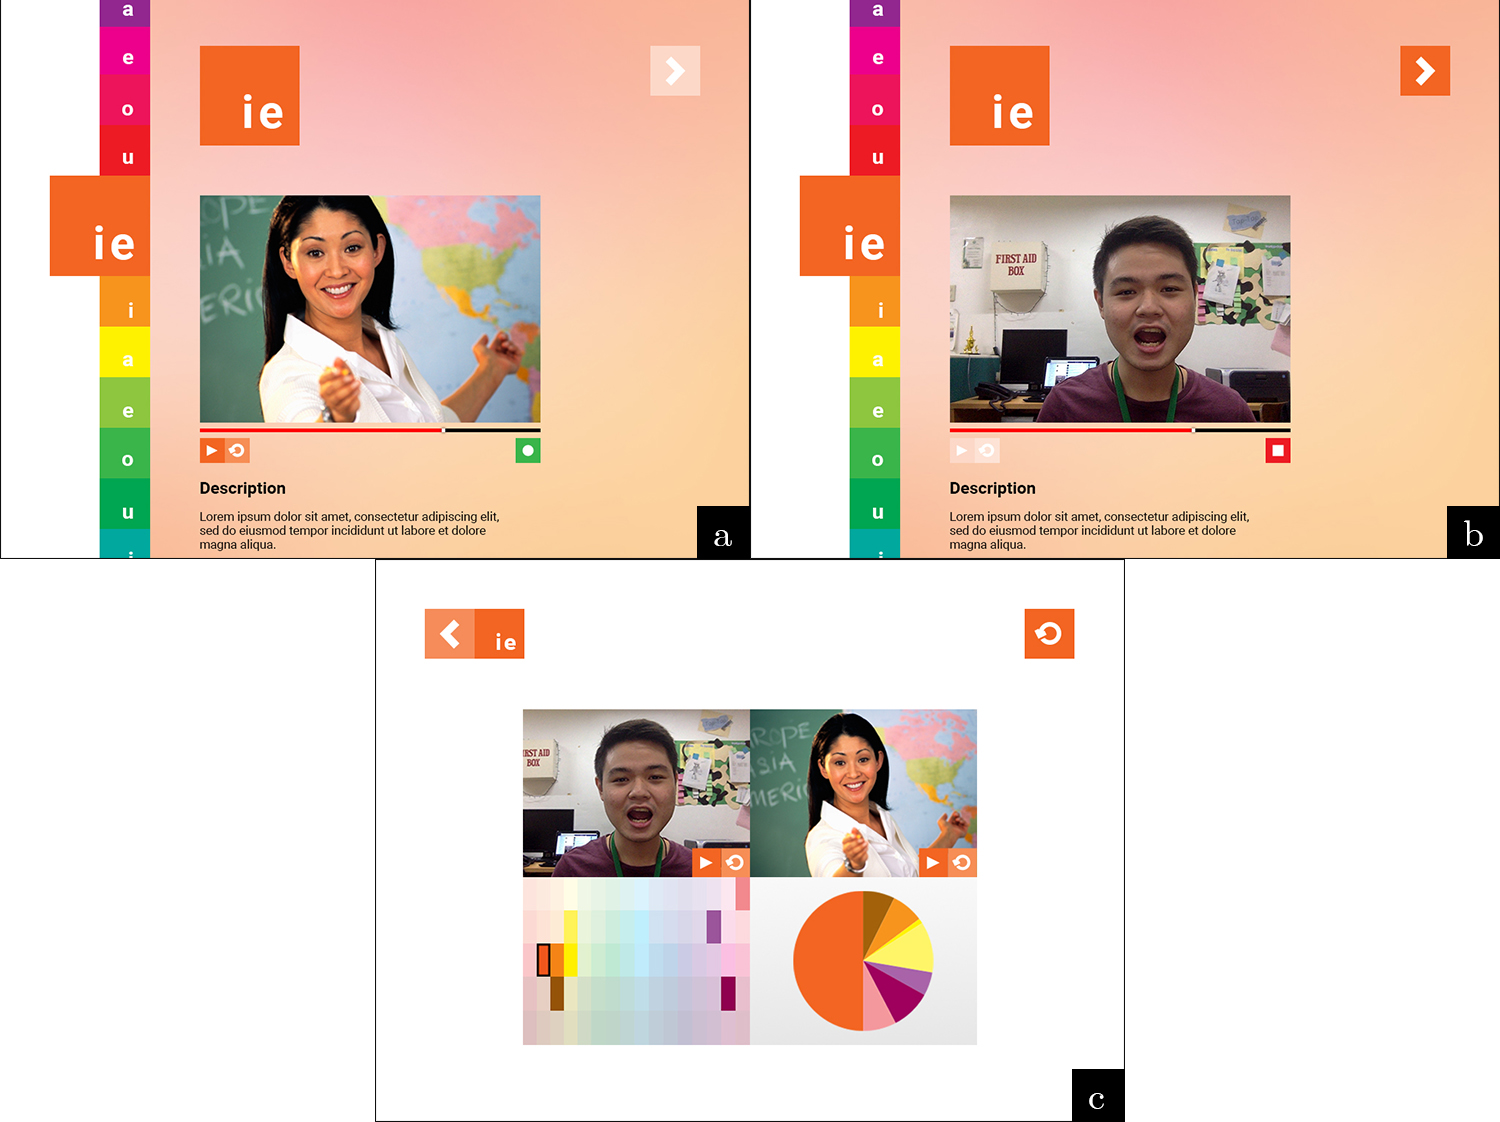
\includegraphics[totalheight=0.5\textheight]{UI}
    \caption{(A) The main menu allows the teacher to select a phoneme for the student to practice. (B) The teacher must record the student's pronunciation through the use of the record button. (C) After recording, the student is shown visual feedback displaying the sound he made in the spectrum along with his mouth movement}
    \label{fig:proto-mainmenu}
\end{figure}


\pagebreak

\section{System Objectives}

\subsection{General Objective}
To implement a feedback system for speech training that provides the user with correct mouth movement of a selected phoneme, to provide the user with a mean to see himself, and to provide measurable visual feedback.

\subsection{Specific Objectives}
\begin{enumerate}
\item To train the SOM into understanding phonemes
\item To provide a visualization that shows feedback of the trainee's pronunciation of a phoneme
\item To deliver a video feedback for the speech trainee to see himself as reference as to how he performs different mouth movements
\item To display a video recording showing the speech trainee on how to perform the mouth movement of a selected phoneme
% \item To record the audio input of the trainee
\item To record a trainee's phoneme pronunciation
\item To have the system analyze the audio recording of the trainee and map it to the SOM
% REMOVE - Sir Sol \item To map the different diphthongs to their own corresponding color in the spectrum
\end{enumerate}

\section{System Scope and Limitations}
% How big is the dataset?
% What accents? Do accents matter?
% Are we going to use Desktop as our platform?
% What are we going to use it with?
% Is it stand-alone? With the assistance of a teacher?
The system will have a fixed set of phonemes to be used for training which will be provided by the institute. The input will be compared only to the existing data, which means it will use the data to map the input as close as possible if it does not have a corresponding phoneme value. 

The system should be used by a trainee alongside a teacher or a speech therapist as the system may not be comprehensible enough to be used by a child alone. Also, the teacher may have to track the progress of their students.

Videos to be played in the system will be recorded videos of real teachers who will demonstrate correct mouth movement to their students. The webcam, designed to act as a student's reflection, should be running above 20 frames per second in order for the student to clearly observe their mouth movement. The webcam's resolution is set to a minimum of 320 by 240 pixels. The microphone requires to have at least 22050 Hz as its sampling rate. The audio is recorded in one channel only---mono. Only visual feedback will be considered in the system however the teacher may or should also provide feedback to their students by giving appraisal.

The visual feedback given by the system will be near real-time. A short delay will happen while the system is processing the phoneme utterance of the trainee before the system displays the visual feedback.

The system will only run on desktop and laptop machines with Java Runtime Environment (JRE) installed. The machine will need to have a microphone and a camera connected to it.

\pagebreak

\section{Architectural Design}

\subsection{Data Training}

\begin{figure}[h]
    \centering
    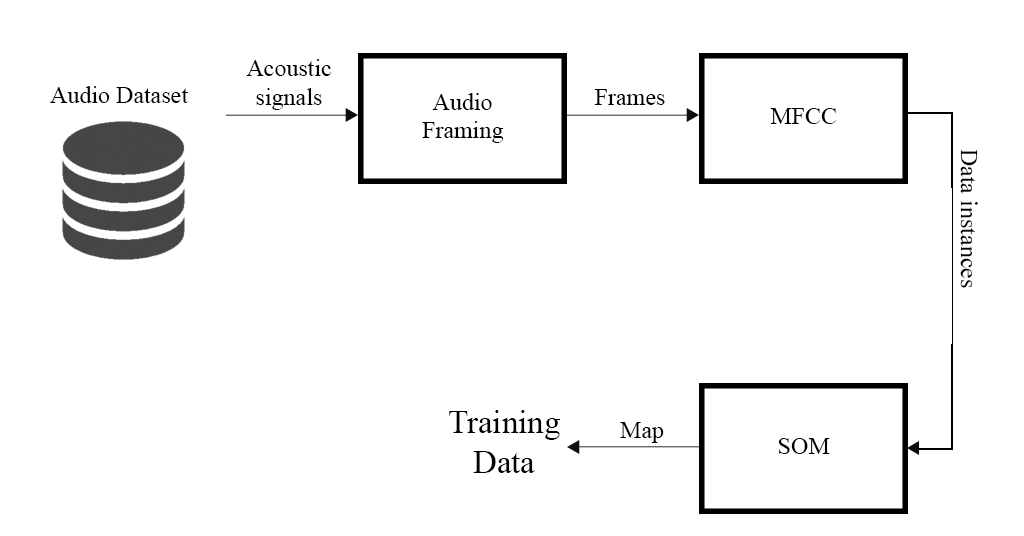
\includegraphics[totalheight=0.3\textheight]{diagram_training.png}
    \caption{System Architecture of the Data Training}
    \label{fig:architecture-training}
\end{figure}

To create a training model containing phonemes for the feedback system, the researchers will adapt to how Agustin's \citeyear{agustin:2014:SOM} created her training model. Recordings of phonemes specified in the scope (see Chapter 1.3) will be collected as training data. Each acoustic signal are then split into frames of 16ms long with 5ms frame shift (defined in 3.2), similar to Agustin's configurations. The first 15 MFC coefficients are computed in each frame. The aforementioned data acquired is then fed into Agustin's SOM which produces a map. Each node of the SOM contains a subset of the whole training data \cite{agustin:2014:SOM}.

\subsection{Feedback System}

\begin{figure}[h]
    \centering
    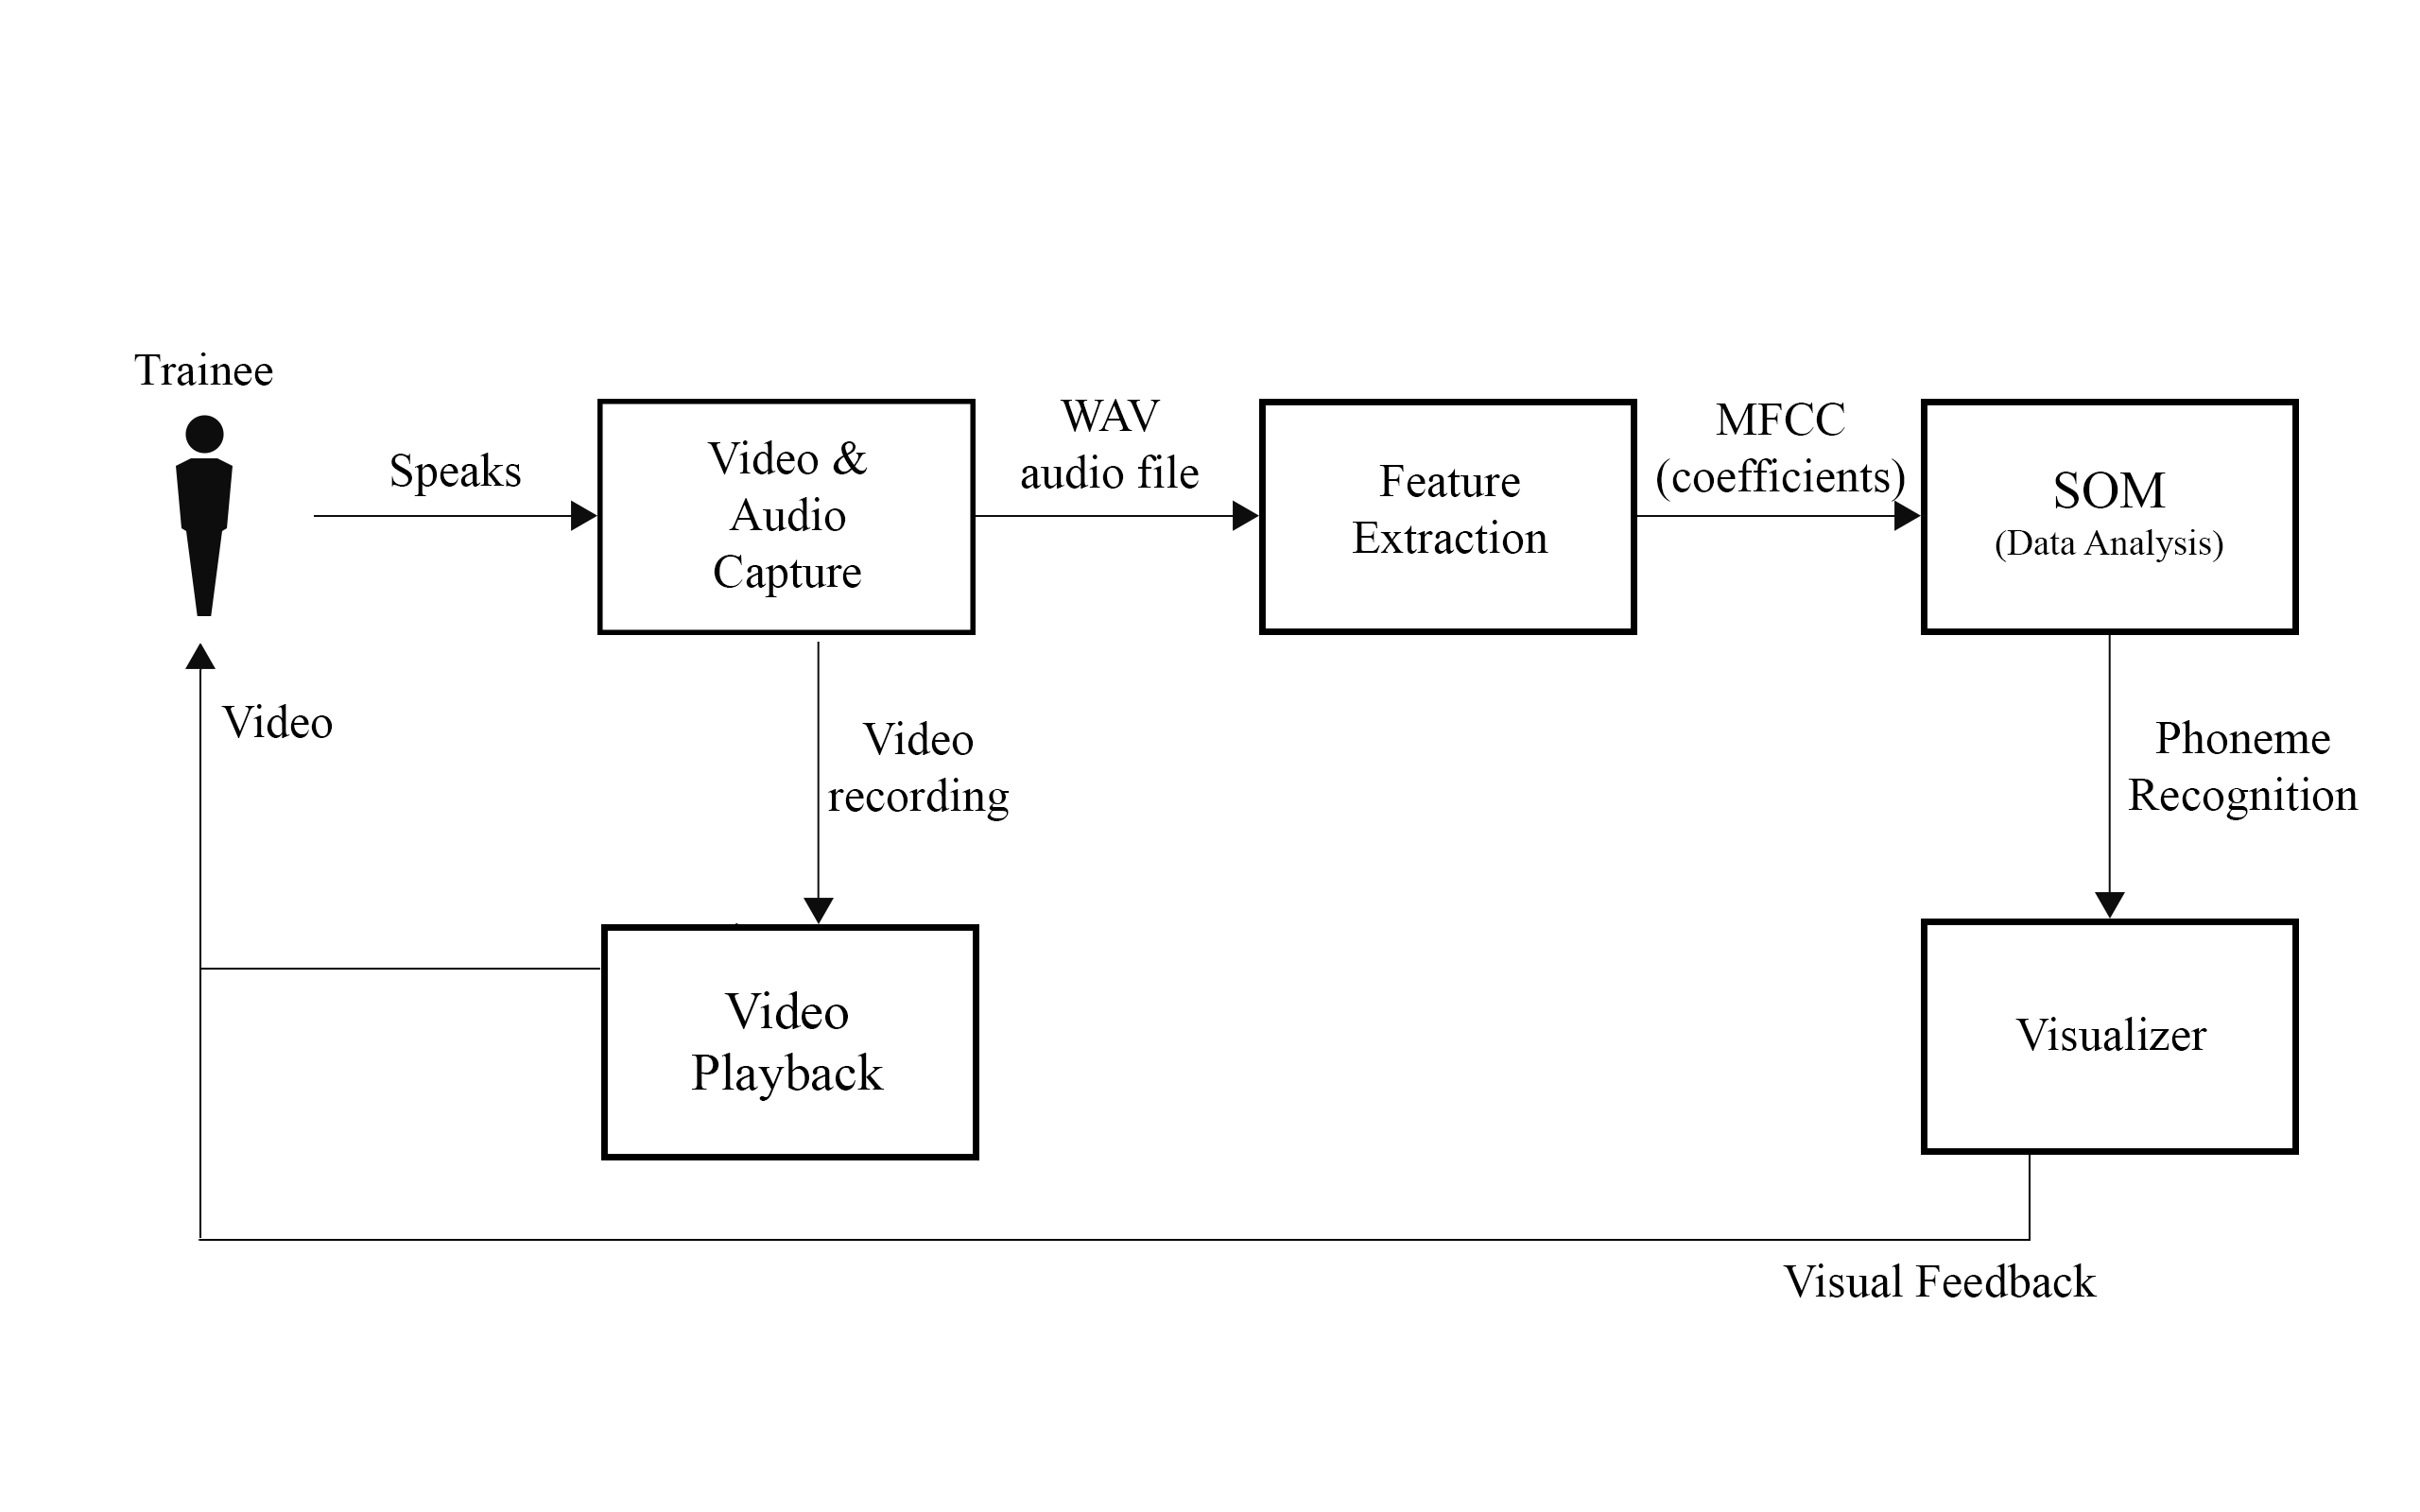
\includegraphics[totalheight=0.3\textheight]{diagram_v3.png}
    \caption{System Architecture of the Feedback System}
    \label{fig:architecture}
\end{figure}

The feedback system is composed of several modules. Each module has a significant responsibility in the feedback system, which greatly helps its users in producing correct speech. A live video camera showcasing the trainee's face will be displayed as well as a video playback of a teacher showing the proper mouth movement when pronouncing the target sound. The trainee interacts with the system in the Audio Capture module. After recording, the audio will go through Feature Extraction using MFCC, which translates important information from the audio into several coefficients. After Feature Extraction, the coefficients will then be laid out on the Self-Organizing Map, which determines how far or how near a trainee is from producing the target sound. The feedback will then be displayed to the trainee.
% Audio Recording -> Feature Extraction (MFCC) -> Mapping (SOM) -> Feedback Display

\section{System Functions}
This section discusses the functions or features available in the speech feedback system.

\subsection{Live Video Display}
For the trainee to see how well he is performing the correct mouth movement when speaking a certain phoneme, the proponents will display a live video display of the trainee which he or she will use for comparison with the recorded video (the correct mouth movement) beside it. This provides Interactive and Mode types of feedback as it visually shows what the student is currently doing.

\subsection{Video Player}
The purpose of the video player is to play a video recording that shows the user on how to correctly pronounce a certain phoneme in which the trainee must imitate. It will be placed beside the webcam display so that the trainee can compare and see if his mouth movement is similar to the video being played. This provides a Mode type of feedback as it shows a visual demonstration of what to do.

%audio record
\subsection{Record Audio}
For the software to process if the trainee's pronunciation is correct, it will need to record the pronunciation of the trainee. After recording, the software will process the voice input in order to display if the pronunciation is correct or not.

\subsection{Feedback Processing}
The software, having performed audio recording, will then process the audio into coefficients following the Mel-frequency cepstral coefficients (MFCC) model, which converts the audio recording into a readable format that will be accepted by the SOM.

After processing the audio and translating it into an array of coefficients, it will then be sent to the self-organizing map (SOM) which will classify the recording and then determine how far or how near the trainee's input is from the target pronunciation.

The software will determine and display how far or how near the trainee's pronunciation is from the target pronunciation through means of color representation. The representation is shown as a color spectrum or a color map. The feedback highlights a targeted color in the spectrum and where the student's pronunciation landed in the spectrum. The student may then keep trying until he gets the correct pronunciation by having the teacher record him again. This presents both the teacher and the student with Amount and Visual feedback (see \figref{fig:feedback-strategy-table} as it shows where and how near or how far the student is from the target pronunciation.

\section{Physical Environment and Resources}

\subsection{Hardware Resources}
The system runs on a desktop or a laptop machine. The system requires a microphone and a web camera connected to it. The minimum supported resolution of the system is 1280x720 pixels. For the system to run smoothly, a machine with a dual-core CPU is needed with at least 2.3 GHz clock speed. At least 4gb RAM is also needed as Java and MATLAB make use of a lot of resources in order to run smoothly.

\subsection{Software}
% JRE 1.8
The machine needs to have the Java Runtime Environment version 1.8 installed for the feedback system to run.
% MATLAB
MATLAB is used to process the audio file (.wav) by using the Mel-frequency cepstral coefficients (MFCC) model which converts audio into coefficients. These coefficients are then passed back to the Java program for processing and analysis.
% VLC
The video player becomes functional when VLC media player is installed in the machine as the feedback system relies on VLC media player's libraries. It is important to take note that if the machine's operating system is 32-bit, then a 32-bit version of VLC media player must be installed. A 64-bit OS will require a 64-bit version of VLC media player.


\appendix
%%%%%%%%%%%%%%%%%%%%%%%%%%%%%%%%%%%%%%%%%%%%%%%%%%%%%%%%%%%%%%%%%%%%%%%%%%%%%%%%%%%%%%%%%%%%%%%%%%%%%%
%
%   Filename    : appendix_A.tex 
%
%   Description : This file is one of the appendices. 
%                 
%%%%%%%%%%%%%%%%%%%%%%%%%%%%%%%%%%%%%%%%%%%%%%%%%%%%%%%%%%%%%%%%%%%%%%%%%%%%%%%%%%%%%%%%%%%%%%%%%%%%%%

\chapter{Diagrams and Other Documentation Tools}
\label{sec:appendixa}

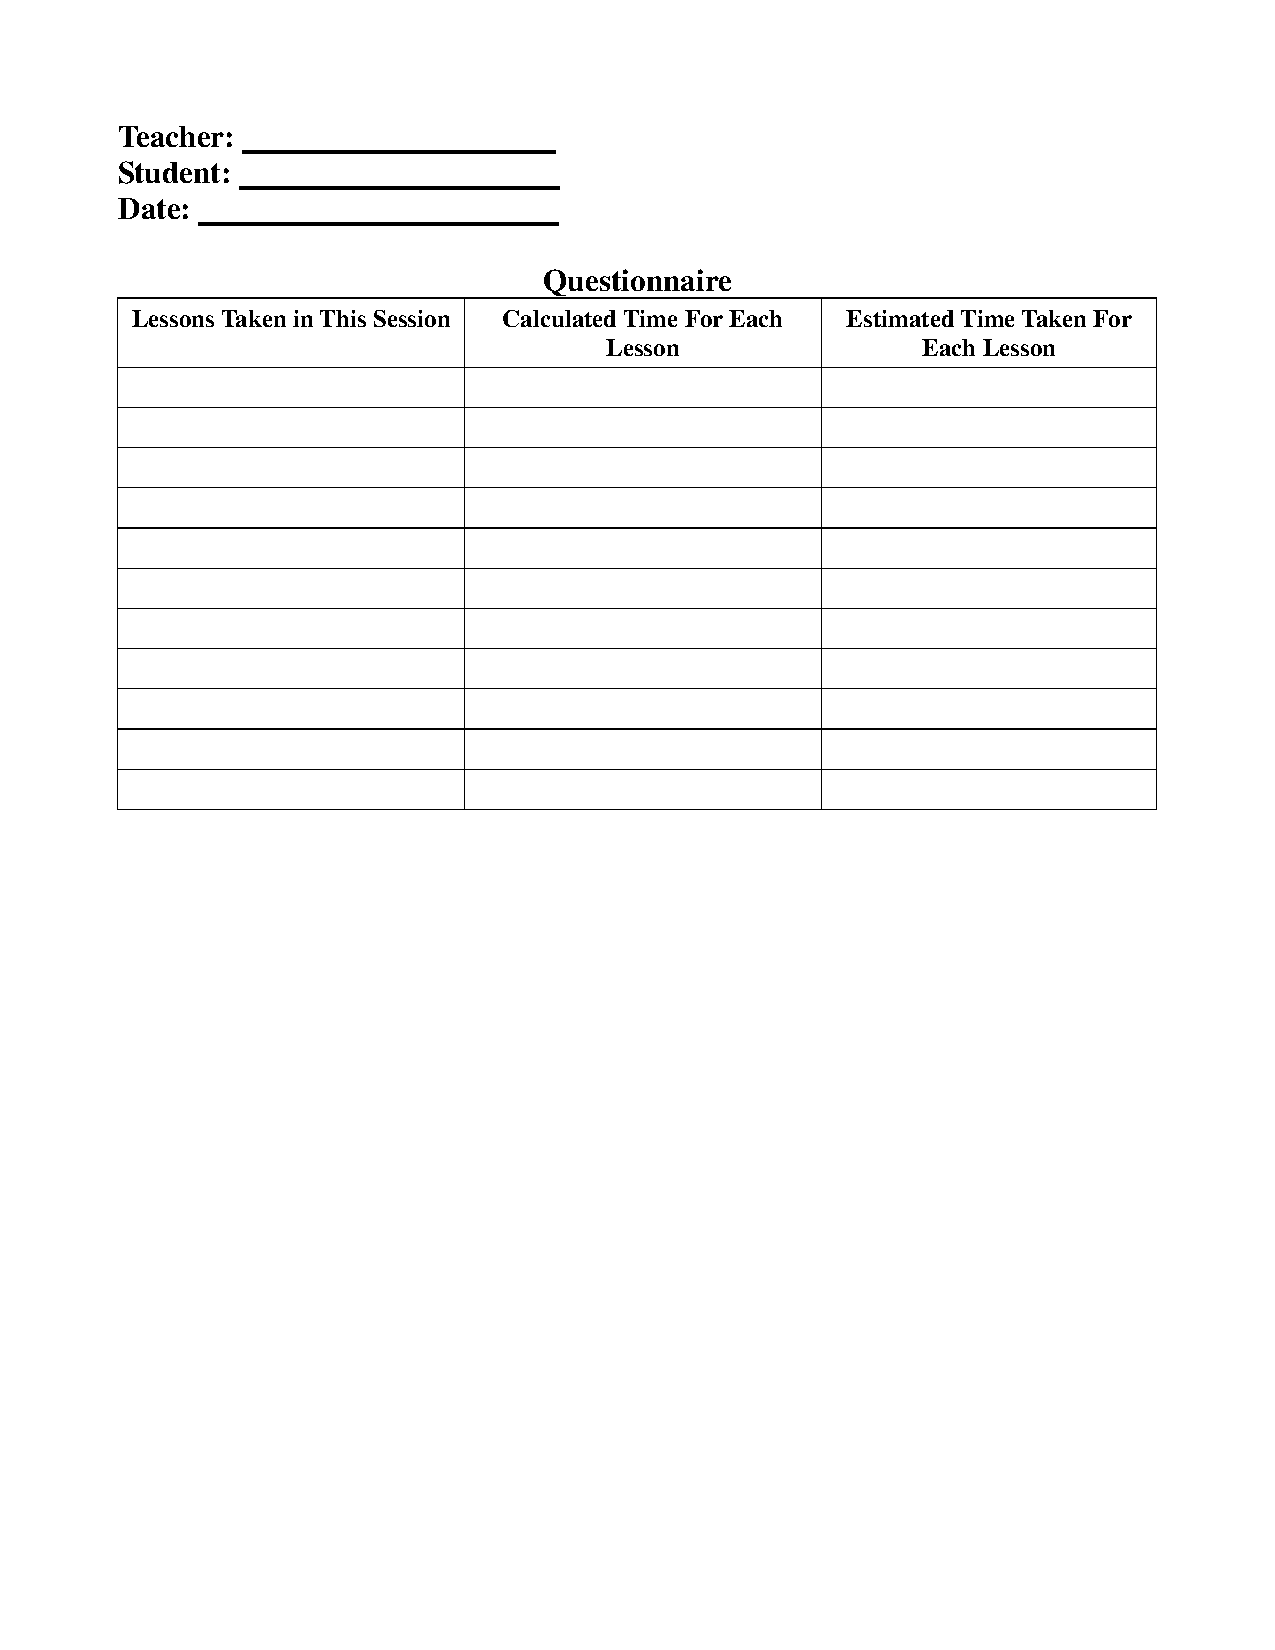
\includepdf[pages=-, scale=.8]{questionnaire.pdf}





\bibliography{references}       %-- the file "myreferences.bib" is a sample bibliography (bib) from SIGGRAPH 
                                  %-- your job: **CREATE/EDIT** your own bibliography file  

\end{document}

